\documentclass[12pt]{article}
\usepackage{graphicx,float,amsmath,amssymb,url}

\makeatletter
\def\ps@pprintTitle{%
 \let\@oddhead\@empty
 \let\@evenhead\@empty
 \def\@oddfoot{\centerline{\thepage}}%
 \let\@evenfoot\@oddfoot}
\makeatother

\DeclareMathOperator*{\argmax}{arg\,max}

\setlength{\parskip}{1em}

\graphicspath{ {../../static/img/}}

\usepackage[backend=biber]{biblatex}
\bibliography{report}

\begin{document}

\section{Introduction}

% The World's Hardest Game~\cite{game} (TWHG) is a widely-available online Flash game known for its infuriatingly difficult gameplay. In the game, a player selects a move from a discrete set (up, down, left, right, stay) to make at each time step, with the goal of navigating through a series of levels. While the game is deterministic (modulo some random initialization of the enemies), it is a very difficult task for humans to complete, requiring precision, patience, and often a difficult-to-discover strategy for movement. However, the set of actions to be taken at any given time step is bounded in size, and the reward for an action is easily calculated. Thus, the game is a good candidate for a reinforcement learning-based model.

The World's Hardest Game~\cite{game} (TWHG) is a widely-available online Flash game known for its infuriatingly difficult gameplay. In the game, a player selects a move from a discrete set (up, down, left, right, stay) to make at each time step, with the goal of navigating through a series of levels. In order to complete a level, the player must collect all on-screen coins, avoid collision with any enemies, and reach the area designated as the end zone. While the game is deterministic (modulo some random initialization of the enemies), it is a very difficult task for humans to complete, requiring precision, patience, and often a difficult-to-discover strategy for movement. However, the set of actions to be taken at any given time step is finite, and the reward for an action is easily calculated. Thus, the game is a good candidate for a reinforcement learning-based model.

\begin{figure}[H]
  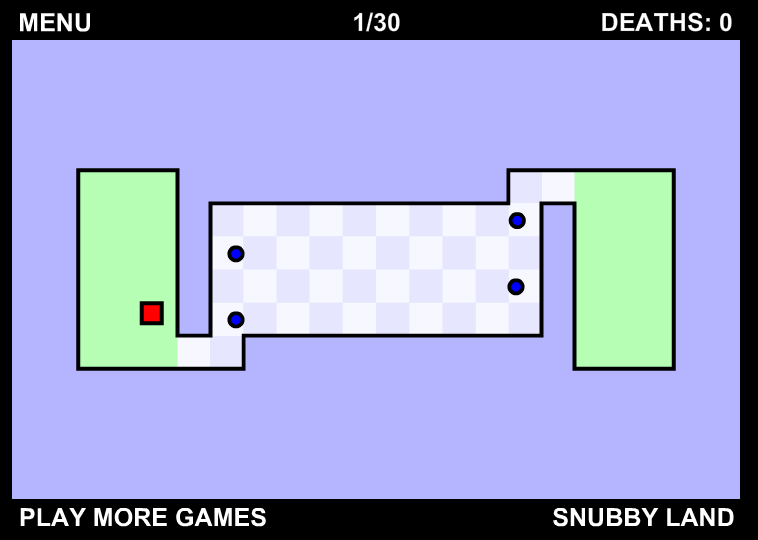
\includegraphics[width=1\textwidth]{report/hardest_game}
  \caption{Level 1 of TWHG}
  \label{fig:twhg}
  \centering
\end{figure}

Deep learning, combined with classic reinforcement learning techniques, allows one to learn a action-selection policy on complicated, long games that have significant delays between action and reward. Furthermore, a CNN is capable of taking pixel inputs from frames of a game simulator and learning a representation of the game state from them. Thus, it is theoretically possible to have a game-winning strategy learned simply by ``playing'' a game over and over, and observing the results.

The original goal of this project was to use the Deep Q-learning with Experience Replay technique pioneered by DeepMind~\cite{deepmind} to train a model that was capable of beating TWHG, surpassing the performance of even the most skilled human player. After weeks of training, it became clear that acheiving this is beyond the scope of the project, with the best models barely managing to navigate the player out of the starting area. Therefore, I instead explored several related ``toy'' games (all with a similar premise), testing the techniques and hyperparameters laid out in the DeepMind paper against two baselines: a random model, and a $\epsilon$-greedy model.

I tested my architechture and model against increasingly complicated toy games, attempting learning both with pixel inputs as well as by directly feeding in a representative state vector. The results show that training with image inputs takes prohibitively long, where as directly feeding in state vectors results in a model that outperforms both the baselines within days. Furthermore, the learned models take actions that are intuitive to a human player, with no seeding required.

\section{Background}

\subsection{Reinforcement Learning}

Q-learning, in which an agent optimizes a game-specific \textit{reward function} by taking an \textit{action} which maximizes the discounted sum of future rewards (\textit{Q values}), is a popular reinforcement learning technique for interacting with an \textit{environment} and set of actions that can be modelled as a finite Markov decision process (MDP). The solution can be discovered via a simple value-iteration update algorithm~\cite{Watkins1992}.

At its heart, the process works as follows. At each time step, the actor selects an action from $\mathcal{A}$, the space of actions available in the given environment $\varepsilon$. This action is passed to a simulator (implemented in our case for each game learned), which modifies $\varepsilon$, without revealing its internal state. The agent then observes state vector representing the $\varepsilon$, as well as a reward $r_t \in \mathbb{R}$. This sequence of actions, observations, and rewards is then used to solve the MDP they represent. Future rewards are discounted by a rate $\gamma$.

\subsection{Deep Reinforcement Learning}

Advances in deep learning have brought about the advent of Deep Q-learning, which relies on the same underlying principles as Q-learning, but replaces the central lookup table with a neural net, allowing one to learn a function apprimator to the $Q$ function in a much larger and sparser action space, without exploring every possible set of moves (which can often be intractable for more complicated games). Furthermore, convolutional layers of the net allow the model to learn directly from game frames (or in our case, several stacked frames), decreasing the amount of structured information that needs to be supplied. This technique was successfully used to play Atari 2600 games at an expert level by the DeepMind team~\cite{deepmind}.

Gradient descent technques were used to optimize the parameters of the network. The architechture was a CNN which took $84 \times 84 \times 4$ vectors, and contained two hidden layers: 16 $8 \times 8$ filters of stride $4$ and 32 $4 \times 4$ filters of stride $2$. This was followed by a 256-node fully-connected hidden layer of ReLU, and an output layer with $|\mathcal{A}|$ linear nodes. This will become the starting point of the models described in this paper.

\subsection{Simulators}

As a Flash-based game, TWHG is easy to simulate. Using headless browser wrappers such as Selenium, it is possible to launch instances of Google Chrome and load the SWF containing the game's code without user intervention. Simulating user moves and extracting state is done through the bare-bones JavaScript API exposed by the Flash runtime~\cite{flashjs}. Internal state can be read using the \texttt{TGetProperty} and \texttt{GetVariable} methods, and written using the corresponding \texttt{Set*} methods. Part of the contribution of this project is a generic Python-based simulator~\cite{simulator} which can interact with Flash-based games and report observable state, as well as capture frames for later processing.

\section{Methods}

\subsection{Games}

In addition to TWHG, described above, I implemented several simple games of varying difficulty, in order to test the efficacy of the techniques and models presented in this project within a limited span of time.

\subsubsection{TG1D}

The first game (TG1D) is a very simple game, involving a 1-dimensional 4-square grid that has one enemy randomly placed on one of the middle two squares. The enemy $e$ appears and dissapears with a random phase, and the goal of the player $p$ is to move from the first square to the last, without ever being in the same square as the in-phase enemy. The possible moves for the player are $\{\text{left}, \text{right}, \text{stay}\}$. The observable state vector $S$ for this game is as follows.

\[S_{x} =
\begin{cases}
  -2 & \text{if } e = x \text{ and } p = x \\
  -1 & \text{if } e = x \\
  1 & \text{if }  p = x \\
  0 & \text{else} \\
\end{cases}
\]

\subsubsection{TG2D}

TG2D is the natural 2-dimensional progression of this simple game. The game is played on a $4 \times 4$ grid, with the starting location for $p$ at $(0, 0)$ and the goal location at $(3, 3)$. A single enemy occupies a random square selected from those that are not the start or goal, with a random phase. The objective is the same.  The possible moves for the player are $\{\text{left}, \text{right}, \text{down}, \text{up}, \text{stay}\}$. $S$ for this game follows as expected from the 1-dimensional case, though it is now a matrix (which is flattened to produce the final state vector).

\subsubsection{TG2D-H}

TG2D-H is the exact same game as TG2D, but with multiple enemies. Each enemy is sampled from the squares remaining after removing the start, goal, and any square that currently has an enemy assigned to it.

\subsection{Learning}

To implement the neural net architechture for this model, I used the popular TensorFlow library. Simple abstractions were build around 2D-convolutional and fully-connected layers, which were strung together to test various architechtures. The output of the net represented the Q-estimate for each action, with the best action defined as $\argmax_{a \in \mathcal{A}} Q_a$. The loss function used for optimization is the mean-squared-error of the Q-estimate predicted for a given action $a$ at time $t$, and the ``realized'' Q-value, which is the known reward for $a$ at $t$ added to the discounted Q-estimate of the best action at the state $t+1$, given $a$ was made at $t$.

\[error formula here\]

The difference in Q-estimate for $t$ and ``realized'' Q-value is clipped to be in the range $[\delta_{-}, \delta_{+}]$, as reccomended by the DeepMind paper, in order to limit the scale of the error gradient. Several values where tried for the bounds of this range. Finally, the Adam optimizer was used to optimize this loss function given the game samples.

Samples were provided using the Experience Replay technique described in the DeepMind paper, with an $\epsilon$-greedy policy for selecting optimal moves (with $\epsilon$ controlling how often random moves were made, in order to force exploration, as opposed to the move suggested by the current Q-estimates).

When feeding in frame images, the architechture used was exactly as described in the DeepMind paper~\cite{deepmind}, with either 3 or 5 output nodes, depending on the game. When feeding in state vectors, we instead use 2 fully-connected hidden layers with 256 ReLU nodes each. Further work could include testing out alternative architechtures, particularly in the latter case.

\subsection{Hyperparameters}

A $\gamma$ value of...

- minibatch size
- epsilon
- delta
- replay memory size
- history size
- images vs state vectors

\section{Results}

\subsection{Baselines}

\subsubsection{Random}

\subsubsection{$\epsilon$-Greedy}

\subsection{Toy Games}

\subsection{The World's Hardest Game}

- not great

\section{Discussion}

\subsection{Challenges}

\section{Conclusion}

\subsection{Further Work}

\pagebreak
\printbibliography

\end{document}
